%!TEX root=paper.tex


\newpage
\subsection{Utilization}
\label{sec:util}

\ins{Knowing how third parties use one's API is difficult even in the case of static dependencies. In the case of services, there is no other way but monitoring service utilization. \tool introduces a series of perspectives on utilization. }

\ins{
  
  The most basic possible view shows the cummulative information about all the endpoints and the number of calls to that endpoint over the lifetime of its tracking as well as in the current day and the last seven days.  
}


  \begin{figure}[h!]
  \centering
  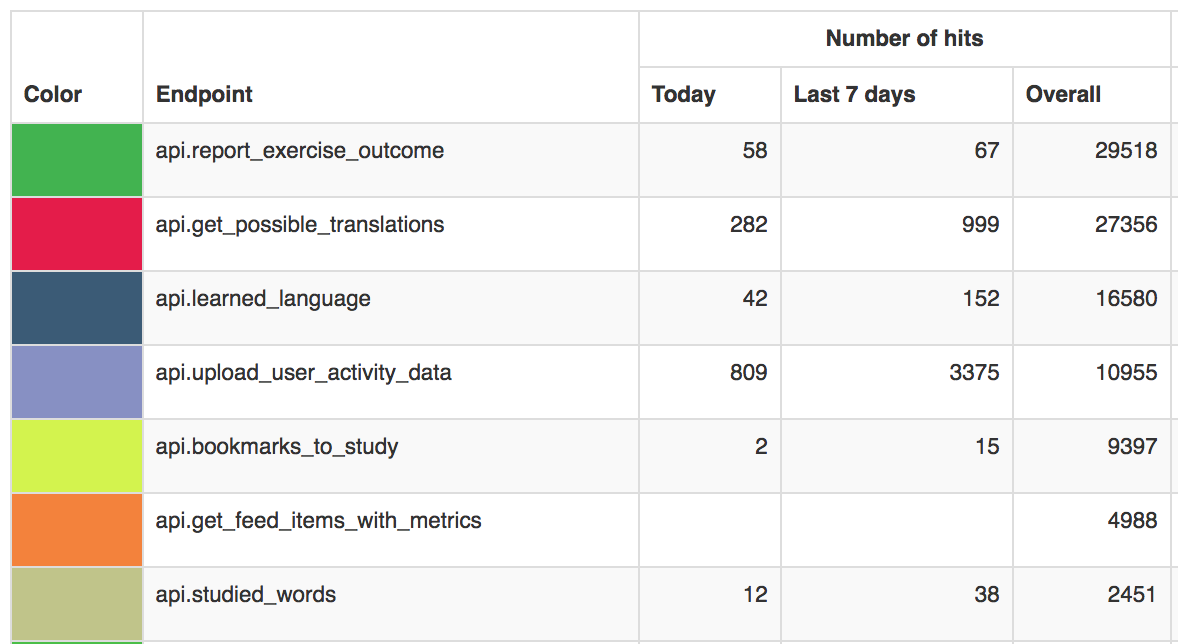
\includegraphics[width=\linewidth]{basicest-utilization}
  \caption{....}
  \label{fig:basicest}
  \end{figure}

This kind of information is already very useful, and can provide the API maintainer with insight into the evolution of their system. By looking at \Fref{fig:basicest}, which presents the top 7 endpoints (for lack of space) one can already see several patterns: 

\begin{itemize}

  \item {\bf Frequent Patterns of System Usage}. The two most used endpoints stand for the two main activities in the system: 

  \begin{itemize}

    \item \epTranslations is an indicator of the amount of foreign language reading the users are doing

    \epOutcome is an indicator of the amount of foreign vocabulary practice the users are doing.

  \end{itemize}

  \item {\bf Sudden Increase of Endpoint Usage}. One endpoint (\epUserActivity) has been disproportionately been used in the last day and last week; much more than before. 

  \item {\bf Possibly Discontinued Endpoint Usage}. One endpoint (\epFeedItems) has not been used in the last 7 days

\end{itemize}

\lesson{Although very useful, it was only after several months of using the system that the client requested the extra columsn for one day and seven days.}

  % \begin{figure}[h!]
  % \centering
  % 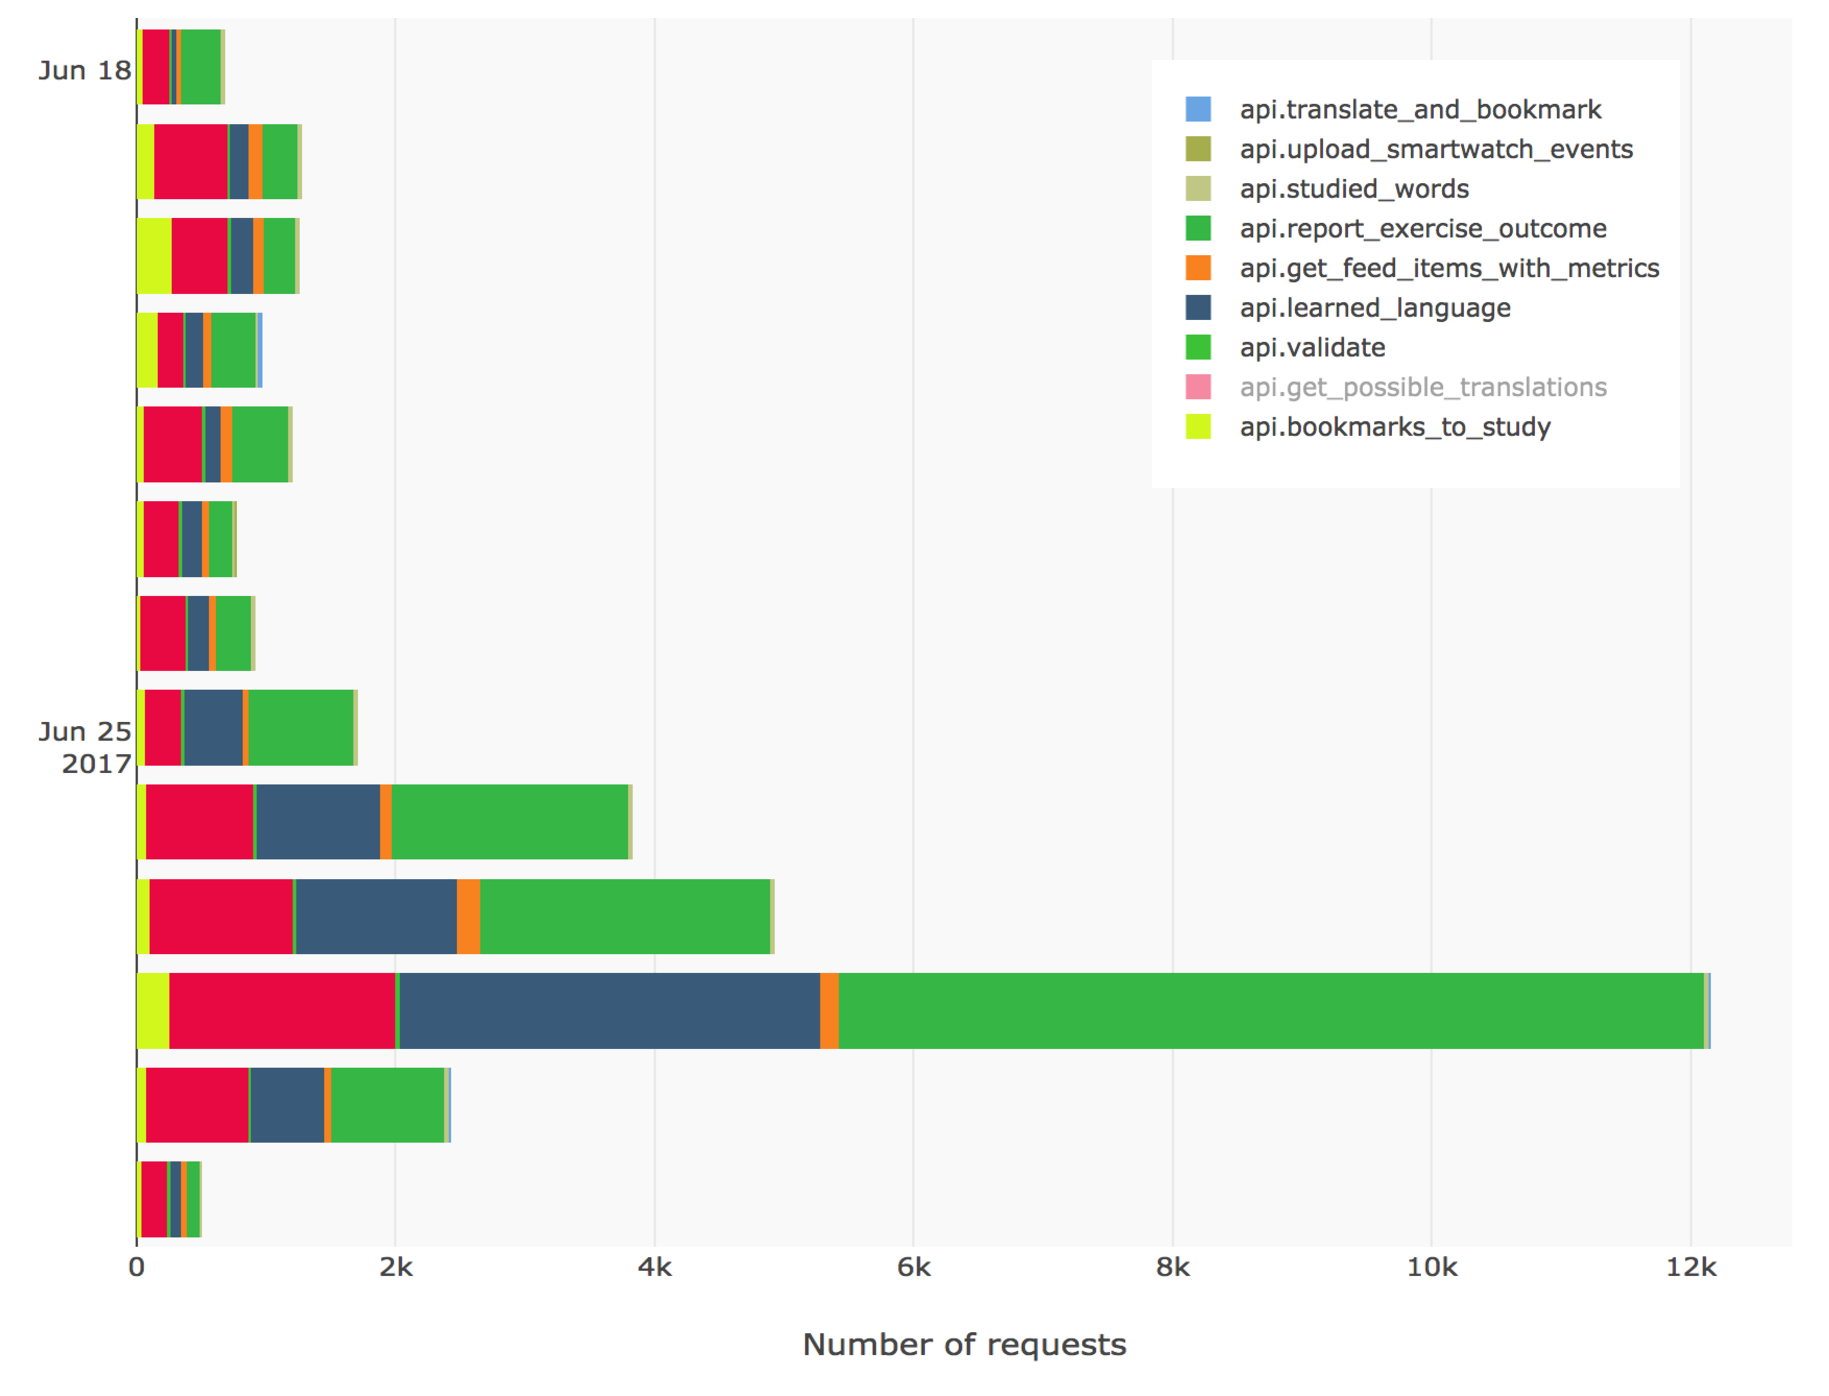
\includegraphics[width=0.5\linewidth]{number_of_requests_}
  % \caption{The number of requests per endpoint per day view shows the overall utilization of the monitored application}
  % \label{fig:aeu}
  % \end{figure}




The table view is limited, and the one day and one week periods are conveniently but arbitrarily selected. For a more detailed evolution of utilization, Figure \ref{fig:aeu} shows the \perspective{Daily Utilization} perspective on endpoint utilization that \tool provides: a stacked bar chart of the number of hits to various endpoints grouped by day\footnote{Endpoint colors are the same in different views}. Figure~\ref{fig:aeu} in particular shows a peak utilization, a day when the API had more than 12.000 hits. 

\begin{figure}[!ht]
\centering
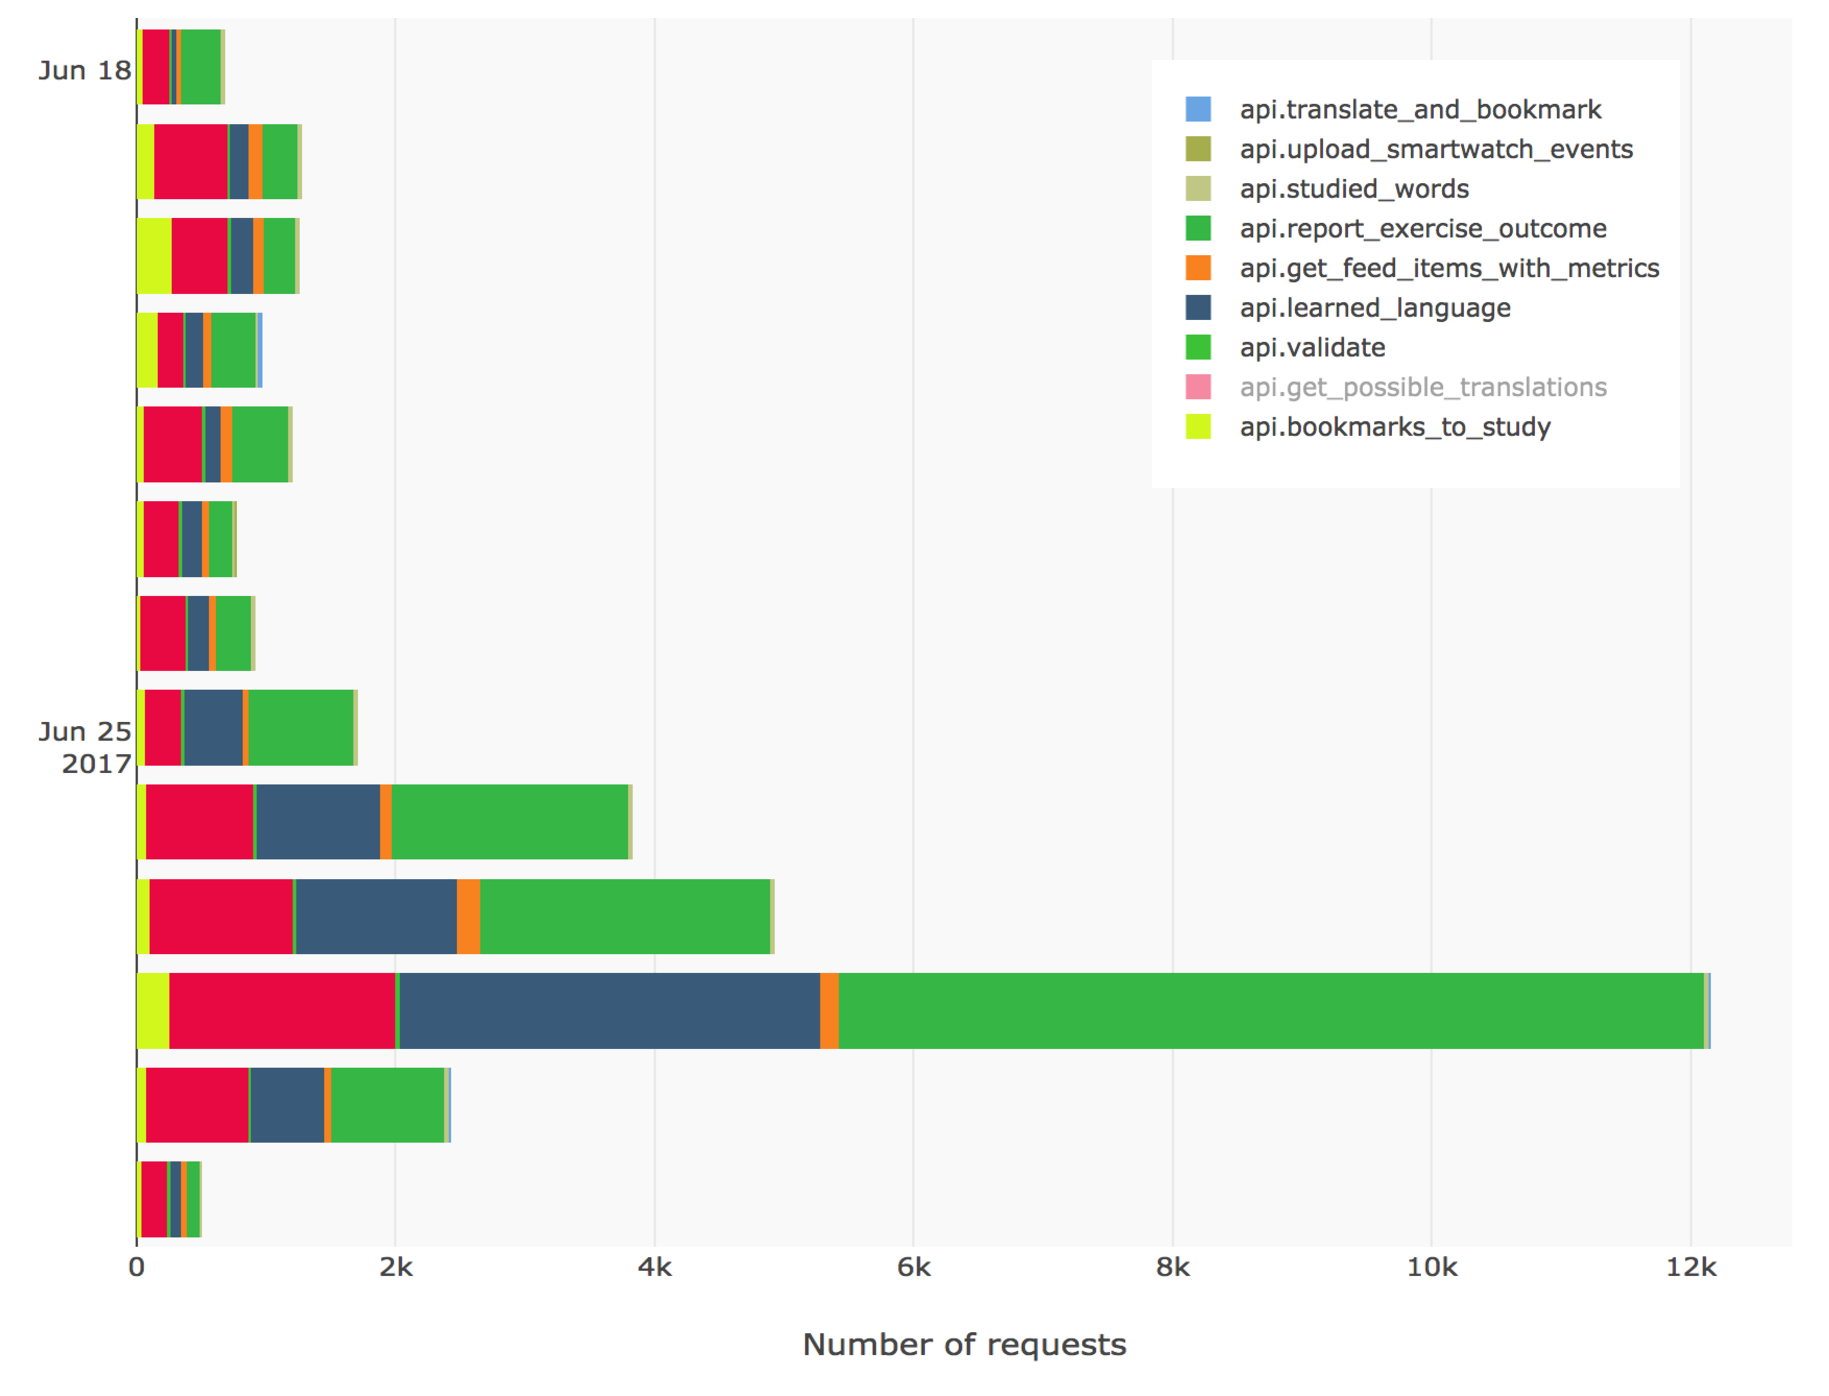
\includegraphics[width=\linewidth]{number_of_requests_}
\caption{Usage patterns become easy to spot in the requests per hour heatmap}
\label{fig:aeu}
\end{figure}


% \begin{figure}[h!]
%   \centering
%   \subfloat[Daily Utilization]{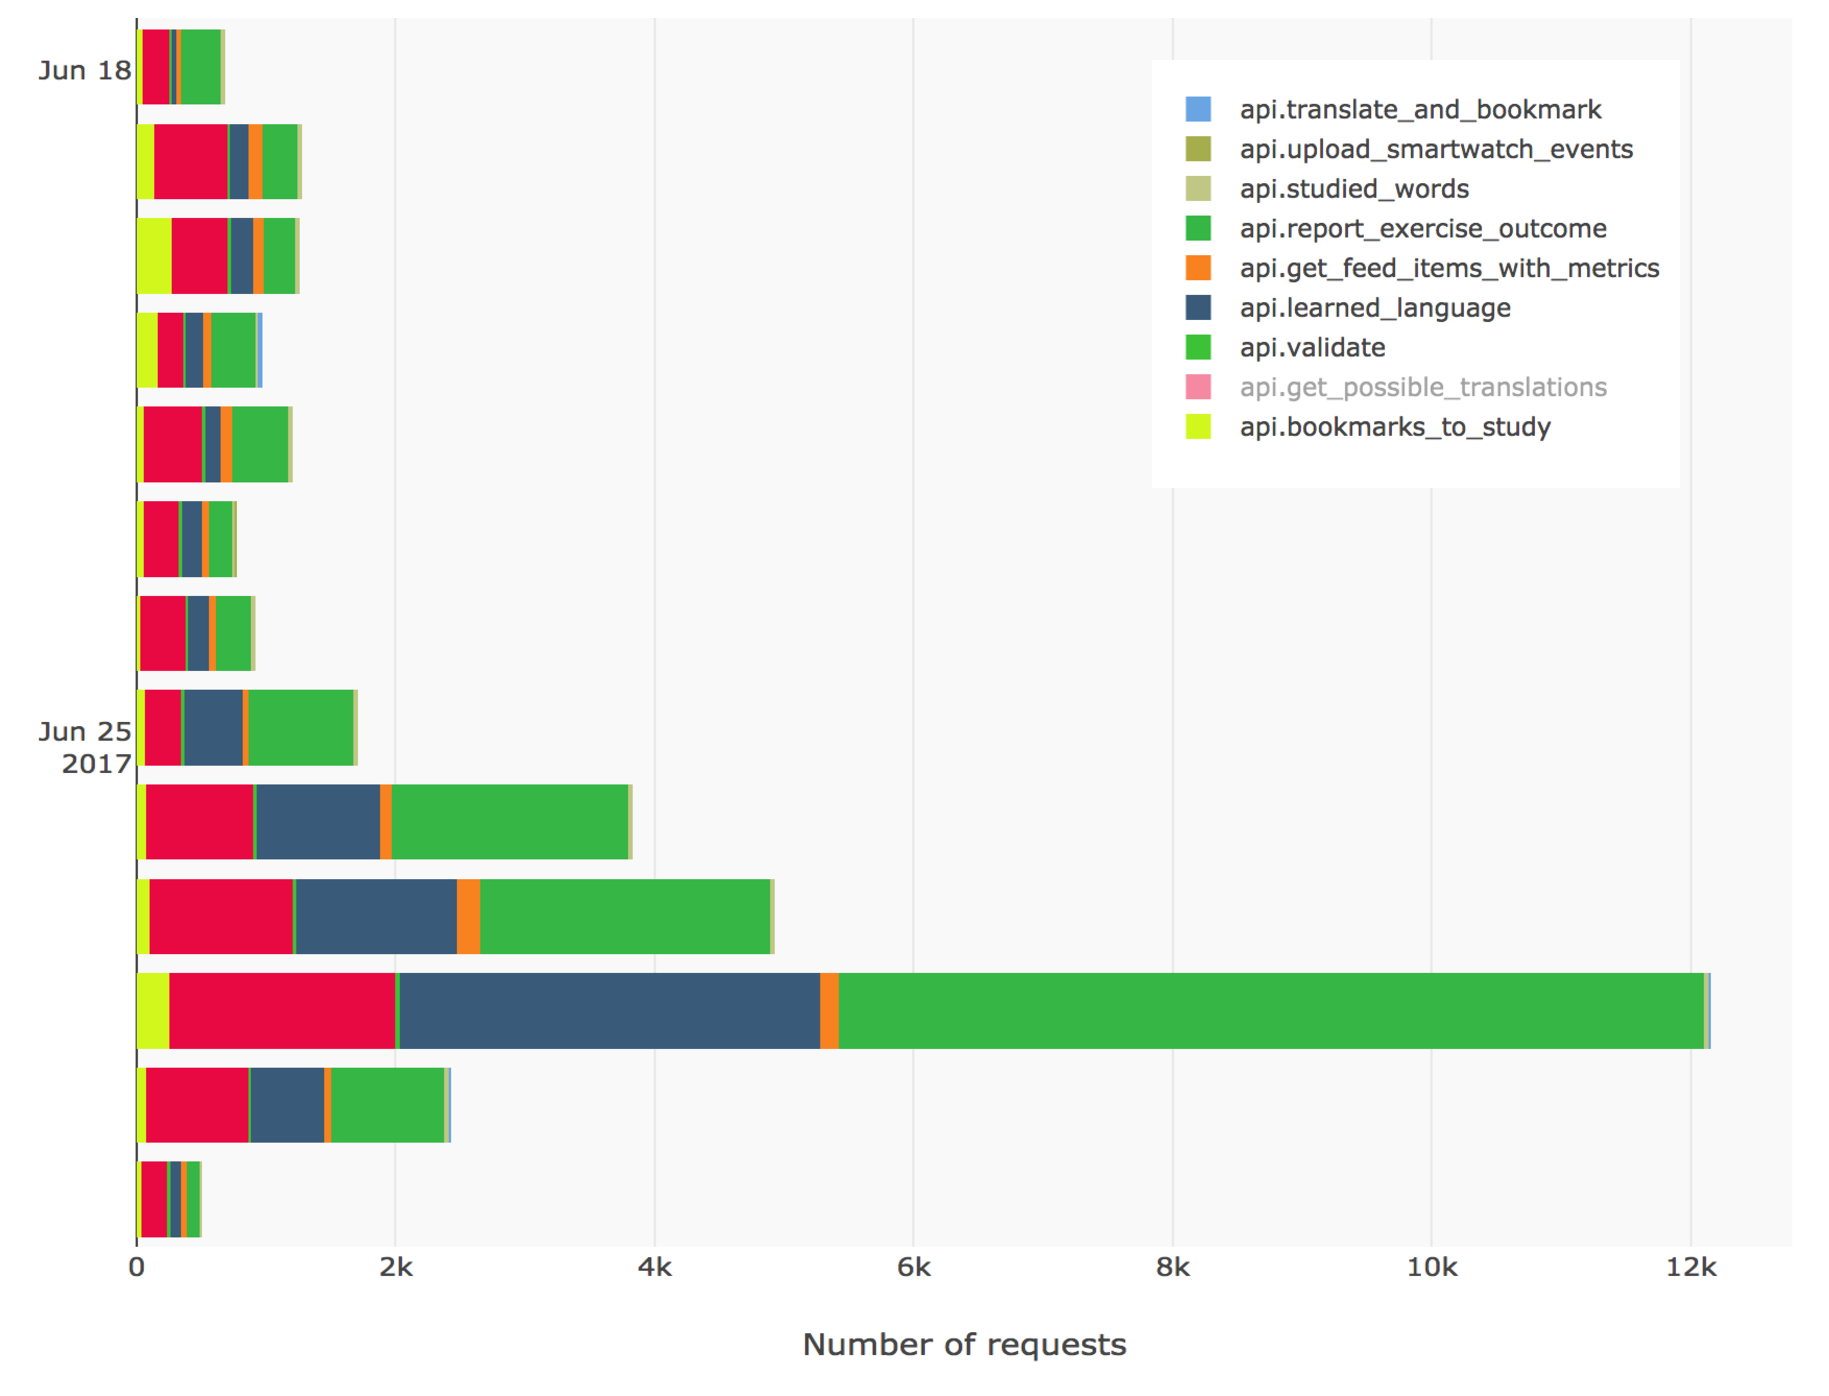
\includegraphics[width=.42\columnwidth]{number_of_requests_}\label{fig:aeu}}
%   \subfloat[Hourly Utilization]{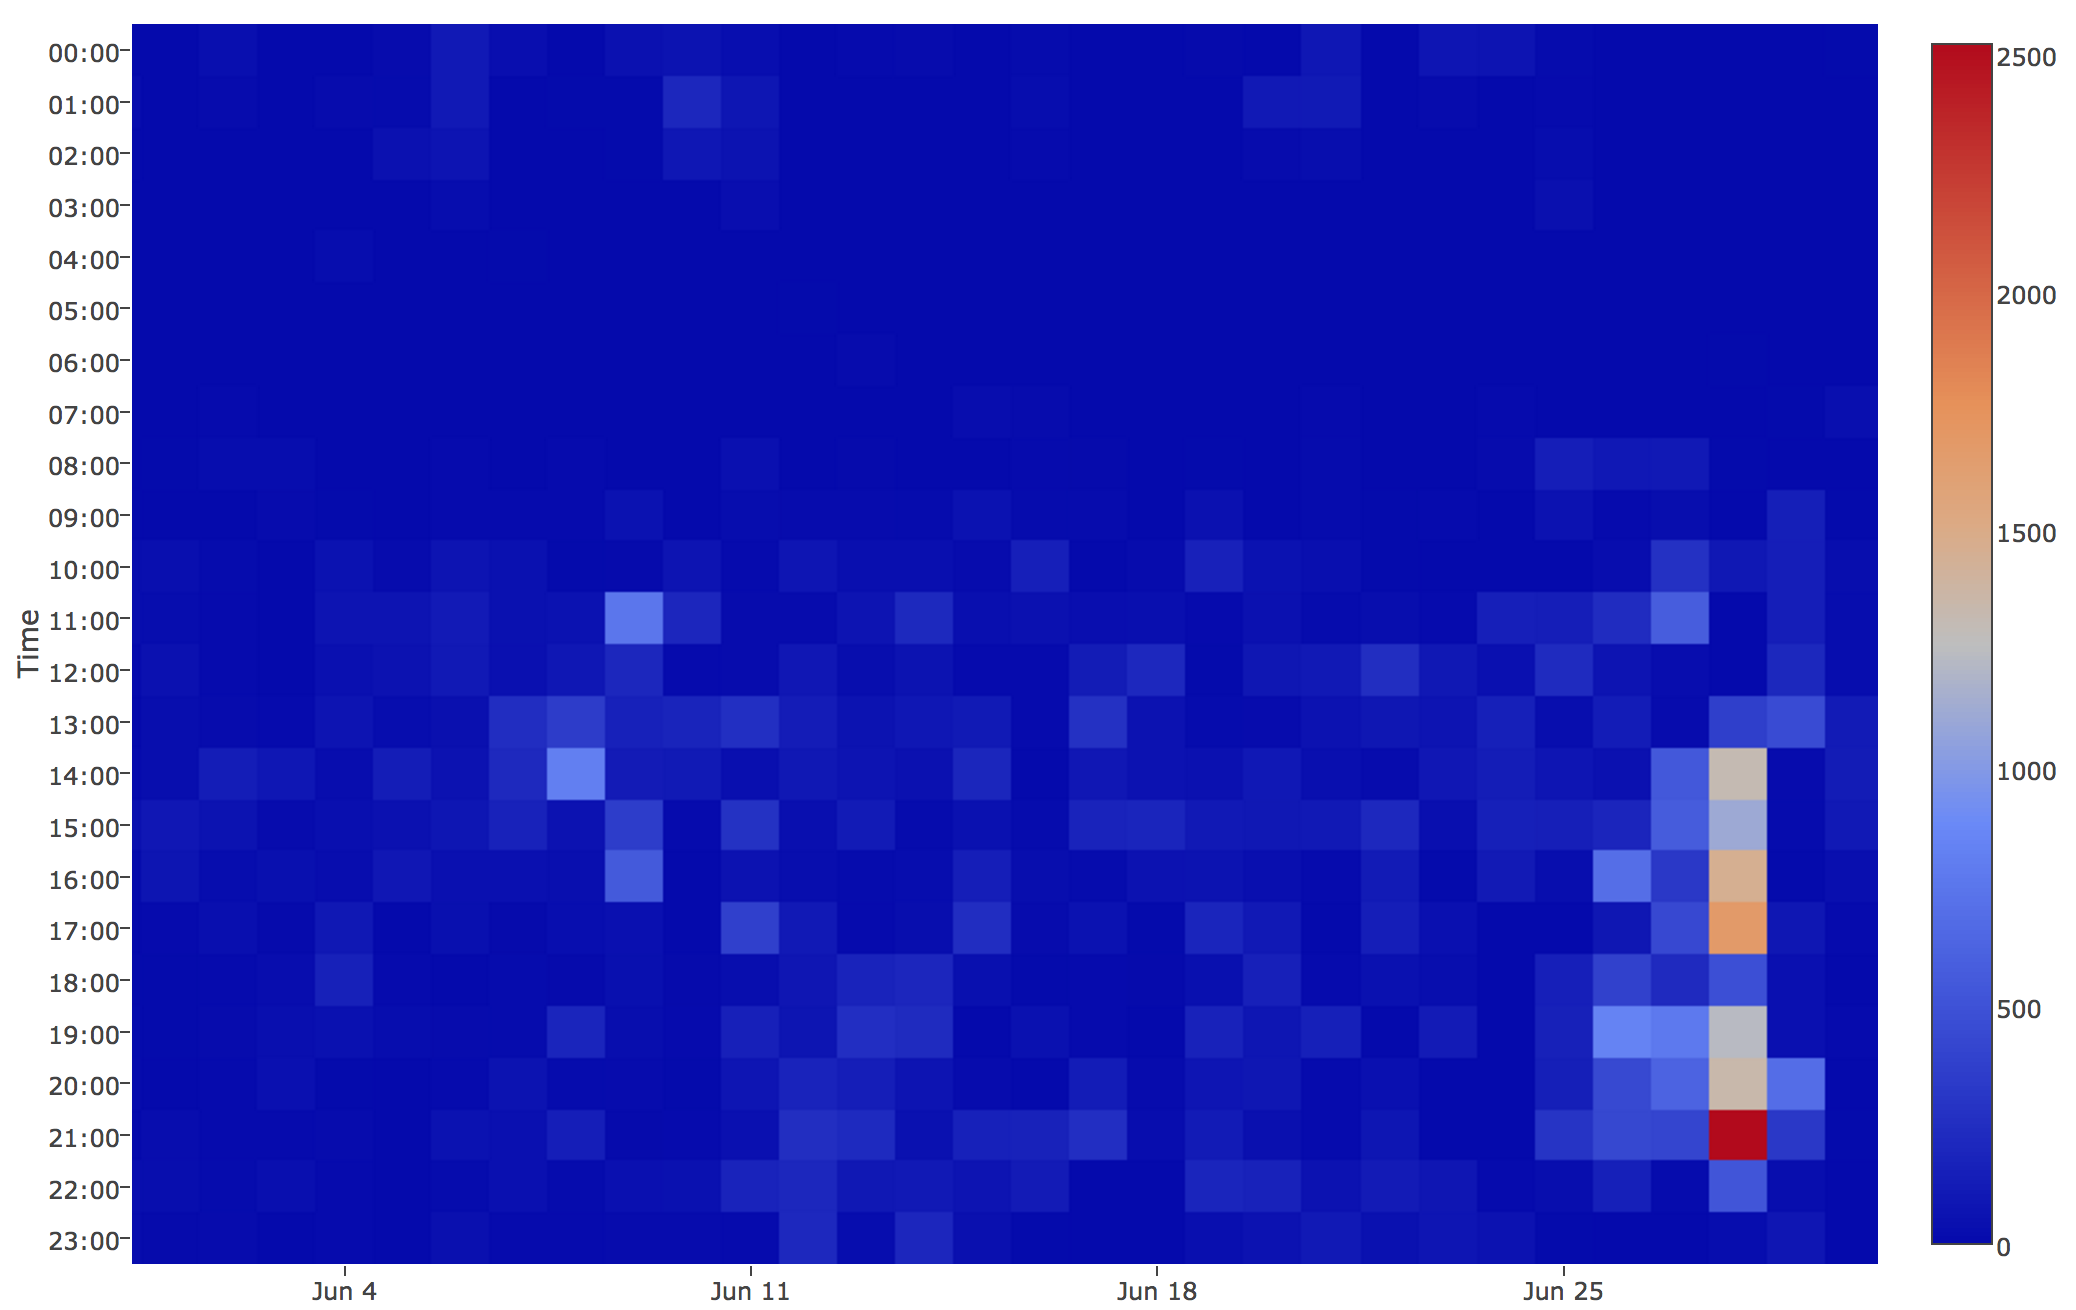
\includegraphics[width=.5\columnwidth]{daily_patterns_}\label{fig:dp}}
%   \caption{Some of the available views\label{fig:views}}
% \end{figure}


% The way users interact with the platform can also be inferred since the endpoints are indicators of different activity types, e.g.: 



% Besides showing the overall utilization, this endpoint provides the maintainer with information relevant for decisions regarding endpoint deprecation --- one of the most elementary ways of {\em understanding the needs of the downstream}\cite{Haen14a}. In our case study, the maintainer realized that one endpoint which they thought was not being used (i.e. \code{words\_to\_study}), contrary to their expectations, was actually being used\footnote{A complementary type of usage information can also be discovered in the view presented in Figure \ref{fig:sep} where seeing that an endpoint is never accessed can increase the confidence of the maintainer that a given endpoint is not used, although it can never be used a proof.}.

% \niceseparator

%   \todo{Add the time series graph and discuss it before the heatmap? We can then sell the heatmap better} 
%   \ml{Not sure about which graph you refer to here V}

Another utilization perspective is the \perspective{Hourly Utilization} in which  the \tool can highlight {\em cyclic patterns of usage per hour of day} by means of a heatmap, as in \Fref{fig:dp}. 


\begin{figure}[!ht]
\centering
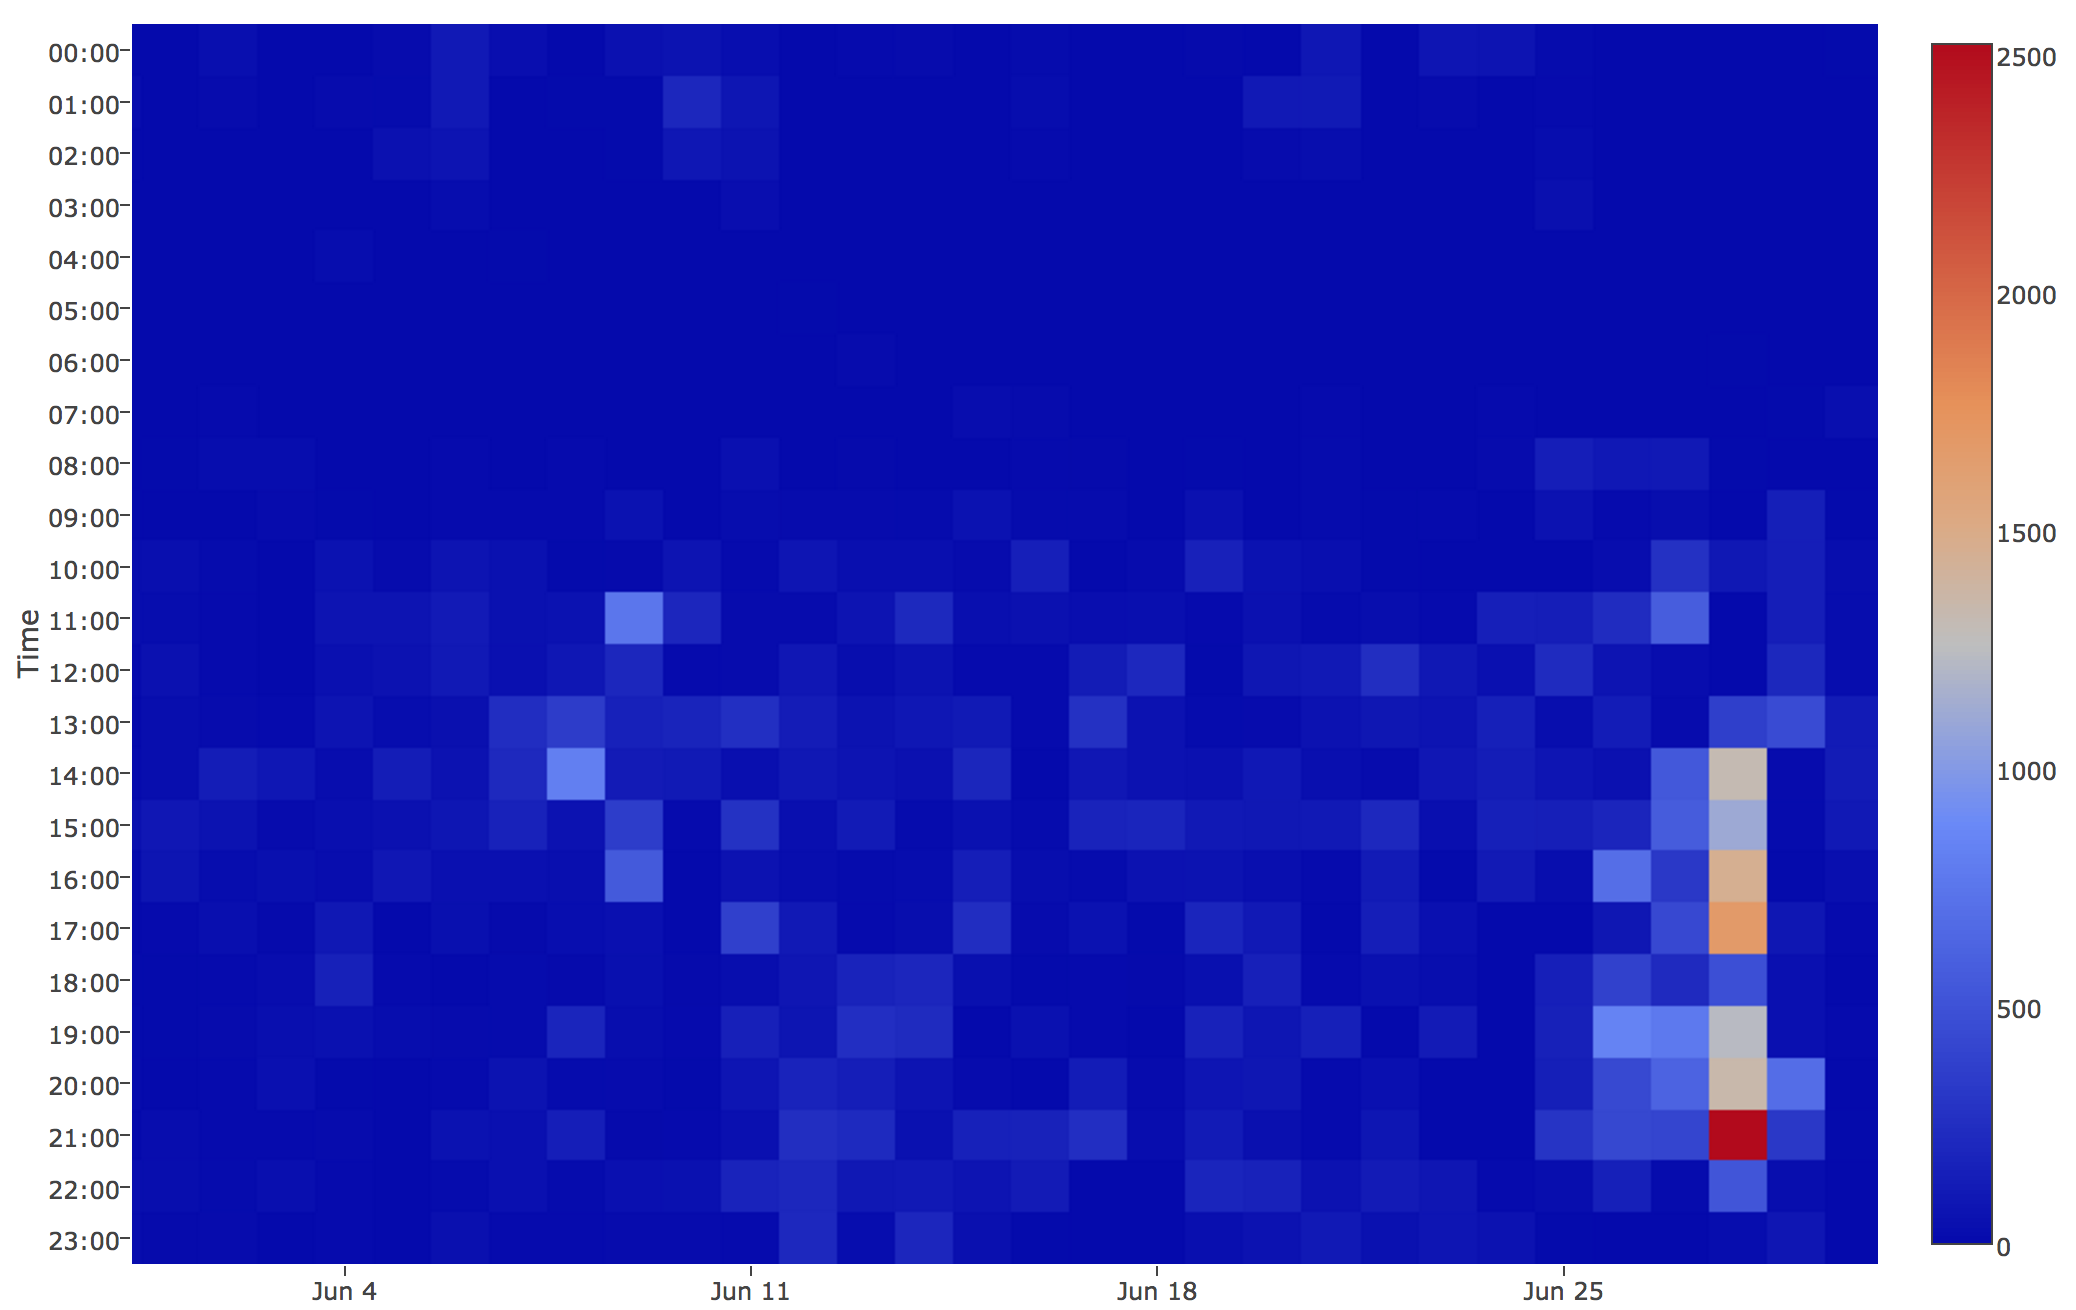
\includegraphics[width=\linewidth]{daily_patterns_}
\caption{Usage patterns become easy to spot in the requests per hour heatmap}
\label{fig:dp}
\end{figure}


Figure \ref{fig:dp} shows the API not being used during the early morning hours, with most of the activity focused around working hours and some light activity during the evening. This is consistent with the fact that the current users are all in the central European timezone. Also, the figure shows that the spike in utilization that was visible also in the previous graph happended in on afternoon/evening.






